%%%%%%%%%%%%%%%%%%%%%%%%%%%%%%%%%%%%%%%%%%%%%%%%%%%%%%%%%%%%%%%%%%%%%%
% How to use writeLaTeX: 
%
% You edit the source code here on the left, and the preview on the
% right shows you the result within a few seconds.
%
% Bookmark this page and share the URL with your co-authors. They can
% edit at the same time!
%
% You can upload figures, bibliographies, custom classes and
% styles using the files menu.
%
%%%%%%%%%%%%%%%%%%%%%%%%%%%%%%%%%%%%%%%%%%%%%%%%%%%%%%%%%%%%%%%%%%%%%%

\documentclass[12pt]{article}

\usepackage{sbc-template}

\usepackage{graphicx,url}

\usepackage[authoryear, round]{natbib}
\usepackage[brazil]{babel}   
\usepackage[utf8]{inputenc}  
 
\sloppy

\title{Proteger para Prevenir: Avaliação de Métodos Anti-Keylogger em Segurança da Informação\\ }

\author{Uriel do C. Andrade\inst{1},\\
Daniel de Oliveira Capanema\inst{1}, \\
Rafael Henriques Noqueira Diniz\inst{1}}


\address{Instituto de Ciências Exatas e Informática\\
Pontifícia Universidade Católica de Minas Gerais (PUC-MG)\\
Caixa Postal 1.686 – 30535.901 – Belo Horizonte – MG – Brasil
\email{uandrade@sga.pucminas.br}
\email{danielcapanema@pucminas.br, 557643@sga.pucminas.br}
}


\begin{document}

\maketitle
\begin{abstract}
    In this article, we analyzed the effectiveness of detection and mitigation tools for \textit{keyloggers}, focusing on solutions that are available and widely used by end users. International tests were conducted on malware that uses heuristics to detect threats, including Windows Defender, Avast, AVG, Bitdefender, MalwareBytes, and AV Total. The results revealed differences in detection efficiency depending on the malicious file format (e.g., \texttt{.exe}, \texttt{.zip}, \texttt{.xlsm}). While some antivirus programs perform well in blocking \textit{keyloggers}, others show significant weaknesses, especially in detecting malicious files and macros. The research highlighted vulnerabilities in these tools and proactively emphasized the importance of raising user awareness and improving security systems to reduce the risks of attacks.
\end{abstract}

\begin{resumo}
    % não é texto de ficção. não tem que ter suspense. Colocar no resumo tudo que foi feito e os resultados.
    Neste artigo, analisamos a eficácia das ferramentas de detecção e mitigação de \textit{keyloggers}, com foco em soluções que estão disponíveis e são amplamente utilizadas pelos usuários finais. Testes internacionais foram realizados em vírus que usam heurística para detectar ameaças: Windows Defender, Avast, AVG, Bitdefender, MalwareBytes e AV Total. Os resultados mostraram diferenças na eficácia da detecção dependendo do formato do arquivo malicioso (por exemplo, \texttt{.exe}, \texttt{.zip}, \texttt{.xlsm}). Embora alguns antivírus façam um bom trabalho no bloqueio de \textit{keyloggers}, outros apresentam sérias fraquezas, especialmente quando se trata de encontrar arquivos e macros maliciosos.  A pesquisa destacou vulnerabilidades nessas ferramentas e reforçou de forma proativa importância de conscientizar os usuários e aprimorar sistemas de segurança para reduzir os riscos de ataques.\end{resumo}
\section{Introdução}

Nos últimos anos, os avanços na área de tecnologia e comunicação deram um grande salto, como a proliferação dos smartphones e a introdução da inteligência artificial no cotidiano. A sociedade moderna encontra-se imersa em um mundo cada vez mais conectado e digital. O acesso facilitado à informação, comunicação e automação tornou-se um dos pilares centrais do mundo tecnológico. No entanto, esses avanços também trouxeram desafios significativos, especialmente no que diz respeito à segurança cibernética.

Neste ambiente dinâmico e em constante evolução, os \textit{malwares} tem sido notícia como uma ameaça à segurança cibernética. Cada avanço tecnológico traz novas falhas de segurança que os malfeitores podem explorar. Seja por rendimentos ilegais, espionagem industrial ou violações de privacidade, os criminosos digitais estão sempre à procura de novas formas de comprometer sistemas e roubar informações sensíveis.

Entre as diversas ameaças que aparecem neste contexto, os \textit{keyloggers} que são uma variante de malwares, destacam-se como ferramentas maliciosas de alta furtividade. Muitas vezes operando em segredo, esses programas capturam e registram cada pressionamento de tecla, expondo usuários a riscos graves, como o roubo de senhas, dados bancários e outras informações confidenciais.

Essa realidade ressalta a importância de compreender as diferentes estratégias utilizadas pelos \textit{keyloggers}, bem como os métodos de defesa disponíveis. A evolução contínua dessas ameaças exige soluções cada vez mais eficazes, capazes de proteger usuários contra ataques cibernéticos em um cenário digital em constante transformação.

\subsection{Problema}

%algum numero que reforce o problema. No mundo 3 bilhões são perdido por ataques. e colocar referência.

Apesar dos inúmeros benefícios proporcionados pelos avanços tecnológicos, os riscos aumentaram proporcionalmente quando o assunto envolve os dados de seus usuários e organizações neste ambiente digital.

\textit{Keyloggers} são uma ameaça crescente que afeta pessoas e organizações em todo o mundo, causando sérios danos e comprometendo informações importantes. De acordo com estatísticas do \citep{securityintelligence2023} do FBI, as perdas com crimes cibernéticos chegarão a USD 10,3 bilhões em 2022, com foco em fraudes de e-mail comercial (BEC) e surtos de ransomware para evitar impactar empresas e usuários finais. O phishing, frequentemente associado a keyloggers, é o crime cibernético mais comum, com mais de 300 mil reclamações recebidas no mesmo ano.

Dada a confidencialidade destes serviços e a sua capacidade de operar em muitas áreas, é importante desenvolver estratégias eficazes para reduzir estes riscos. É importante analisar e comparar métodos de combate aos \textit{keyloggers} para garantir que os benefícios desta ferramenta não sejam comprometidos pelos perigos que pode causar. Compreender os perigos destes riscos e implementar medidas de segurança fortes é crucial para proteger dados e informações importantes.

\subsection{Objetivo principal}
O objetivo principal deste trabalho é investigar detalhadamente o funcionamento de \textit{keyloggers} e realizar uma análise comparativa entre diferentes métodos de detecção e mitigação. Busca-se compreender o comportamento desses programas maliciosos e avaliar a eficácia de cada método na identificação e neutralização de \textit{keyloggers}. Por meio de um ambiente controlado, pretende-se fornecer uma visão clara sobre quais abordagens são mais eficazes para proteção contra essa ameaça.

Esta análise será conduzida comparando diversas ferramentas de proteção, avaliando aspectos como eficiência na detecção, impacto no desempenho do sistema, facilidade de uso, frequência de atualizações, e modelo de licenciamento. Dessa forma, o estudo pretende identificar as soluções mais completas e acessíveis, visando fortalecer as estratégias de segurança digital tanto para profissionais quanto para usuários comuns.

\subsection{Objetivos específicos}

Os objetivos específicos desta pesquisa são:
\begin{itemize}
    \item Criar um ambiente controlado para analisar os mecanismos de operação dos \textit{keyloggers}, observando como eles capturam dados e se mantêm ocultos.
    \item Identificar e avaliar a eficácia de diversos métodos de detecção e mitigação de \textit{keyloggers}, considerando diferentes abordagens técnicas.
    \item Realizar uma análise comparativa entre os métodos de detecção, destacando quais são mais eficientes na prevenção de \textit{keyloggers} em diferentes cenários.
    \item Fornecer recomendações baseadas em resultados empíricos sobre as melhores práticas e estratégias para a detecção e neutralização de \textit{keyloggers}, contribuindo para o aprimoramento da segurança digital.
\end{itemize}

\subsection{Contribuições Esperadas}
A partir da elaboração do trabalho e obtenção dos resultados, espera-se que este estudo contribua para a comunidade técnica e científica ao oferecer uma análise detalhada da eficácia de métodos \textit{anti-keylogger}. Dado que as pesquisas sobre este tema, especificamente em sistemas operacionais de uso comum, são limitadas, este trabalho possibilitará a comparação entre diferentes ferramentas de detecção e mitigação de \textit{keyloggers}, oferecendo insights sobre as soluções mais eficientes para o problema em questão.

\section{Fundamentação teórica}

\subsection{Segurança da informação}
A segurança da informação é uma preocupação crítica para organizações no cenário digital contemporâneo. Como destaca \citep{bhaharin2019issues} , a proteção e segurança das informações organizacionais têm se tornado cada vez mais desafiadoras na era da Indústria 4.0. Isso é atribuído ao surgimento de ameaças sofisticadas à segurança.

O surgimento da Indústria 4.0 trouxe conectividade sem precedentes e integração de tecnologias digitais nos processos organizacionais. Embora essa conectividade tenha facilitado a eficiência e a inovação, também expôs as organizações e seus usuários a uma ampla gama de ameaças cibernéticas. Desde software malicioso e ataques de \textit{phishing} até violações de dados e ameaças internas, o cenário de ameaças moderno é caracterizado por sua complexidade e diversidade.
\subsection{\textit{Malware}}
\textit{Malwares}, abreviação de \textit{malicious software} (software malicioso), é definido pelos autores \citep{singh2021keylogger} como:"\textit{qualquer código ou programa escrito por hackers com a intenção de causar danos a um sistema sem o consentimento do usuário}", ele representa uma ameaça complexa e crescente no mundo digital.

Nesse mesmo contexto, \citep{singh2018infringement} nos traz a informação com relatórios científicos e empresariais, que aproximadamente 1 milhão de arquivos de \textit{malware} são criados todos os dias, e o crime cibernético prejudica a economia mundial em aproximadamente US 6 trilhões anualmente até 2021.

\subsection{\textit{Keylogger}}
De acordo com \citep{wajahat2019novel}, \textit{um \textit{keylogger} são uma ferramente de monitoramento que possui uma certa ou total capacidade de capturar cada pressionamento de tecla de um teclado e armazenar em arquivos de log.}

Também conhecidos como registrador de pressionamentos de tecla, os \textit{keyloggers} é um tipo de \textit{spyware}, que podem ser utilizados tanto em contextos éticos quanto em situações que desconsideram a ética. Em contextos éticos, eles são empregados em empresas onde \textit{"o monitoramento é um fator importante para manter a estabilidade da rede"} \citep{tuli2013system} e para realizar a vigilância de crianças na navegação à internet. No entanto, em cenários onde a ética não é levada em conta, \textit{keyloggers} podem ser usados de forma maliciosa para roubo de informações pessoais, como senhas e dados bancários, espionagem ou outras atividades ilícitas.

Existem dois tipos principais de variações dessa ferramenta, cada uma com suas peculiaridades e mecanismos de funcionamento distintos. O primeiro tipo é o \textit{keylogger} de hardware, \textit{}\citep{singh2021keylogger}. Após os dados serem salvos na memória interna eles podem ser acessados de várias maneiras, dependendo do design do dispositivo e das intenções do atacante.

O segundo tipo é o de software, um programa que é instalado no sistema do computador. \textit{O keylogger de software intercepta dados que viajam pelo teclado e pelo sistema operacional. Ele coleta eventos de pressionamento de tecla, armazenando-as em um local remoto e depois os transmite ao invasor que instalou o keylogger.} \citep{ahmed2014survey}

\subsection{Heuristicas de detecção}
Heurísticas de detecção são técnicas avançadas usadas para identificar ameaças que não são detectadas por métodos tradicionais. Algumas das principais são:

Técnica de anti-hook: "Esta tecnologia é baseada no uso de ganchos de API, que são utilizados por todos os processos (visíveis ou ocultos) para implementar ganchos. Hooks são um conjunto de métodos usados para alterar o comportamento de um sistema operacional ou aplicativo. Isto pode interromper o fluxo de chamadas de função ou mensagens entre diferentes componentes do computador. O sistema verifica todos os processos, executáveis estáticos e DLLs (bibliotecas de vínculo dinâmico) para identificar processos ou arquivos suspeitos que usam ganchos."\citep{solairaj2016keyloggers}

Técnica HoneyID: Descrito como uma ferramenta capaz de "atrair e capturar o invasor" \citep{10124477}, servindo para enganar e monitorar suas atividades. Ele opera como um honeypot, criando iscas no sistema para atrair invasores, registrando suas interações suspeitas e coletando informações sobre seus comportamentos.

Detecção Baseada em Assinaturas: \textit{É um recurso de malware que encapsula a estrutura do programa e identifica cada malware exclusivamente. A abordagem de detecção baseada em assinatura é amplamente usada em antivírus comerciais. Essa abordagem é rápida e eficiente para detectar malware conhecido, mas insuficiente para detectar malware desconhecido.} \citep{aslan2020comprehensive}

\section{Trabalhos relacionados}

A análise sobre a ação dos \textit{keyloggers} fornece uma visão detalhada sobre a definição, os diferentes tipos e as técnicas de detecção e prevenção, conforme discutido por \citep{singh2021keylogger}. O autor aborda amplamente a importância de proteger informações confidenciais contra esses programas maliciosos e apresenta métodos proativos, como o uso de softwares \textit{anti-malware} e a verificação de entradas de inicialização. O trabalho também destaca estratégias específicas para dispositivos móveis, considerando suas características distintas.

Focando em \textit{keyloggers} de software, \citep{wajahat2019novel} aprofundaram a análise de suas operações tanto em modo kernel quanto no espaço do usuário, ilustrando exemplos históricos de uso malicioso, como o roubo de credenciais bancárias. Esses autores propuseram uma solução baseada na simulação de teclas e padrões de entrada/saída, demonstrando eficácia na detecção e aplicabilidade prática, especialmente em dispositivos móveis.

Para \citep{solairaj2016keyloggers} uma ampla gama de técnicas de detecção, incluindo abordagens baseadas em assinaturas e comportamentos, como Anti-Hook e HoneyID. Além disso, propuseram o uso de Support Vector Machines (SVM) para aprimorar a detecção de \textit{keyloggers}. Essa técnica, particularmente relevante para dispositivos móveis, mostrou-se eficaz na superação de desafios específicos, proporcionando maior precisão na identificação de ameaças. Por outro lado, \citep{aslan2020comprehensive} voltaram-se para métodos avançados de detecção de \textit{malware}, como o aprendizado profundo, aplicando-os ao combate de \textit{keyloggers}. A pesquisa evidenciou o potencial dessas técnicas para identificar padrões complexos e oferecer soluções robustas e adaptáveis a diferentes plataformas, com especial foco em dispositivos móveis.

Avanços significativos têm sido feitos na detecção e bloqueio de \textit{keyloggers} nos últimos anos. Estudos como os de \citep{singh2021keylogger}, \citep{wajahat2019novel}, \citep{solairaj2016keyloggers} e \citep{aslan2020comprehensive} destacam técnicas inovadoras nessa área. Este trabalho, no entanto, foca na avaliação de ferramentas que utilizam essas técnicas, priorizando sua acessibilidade e eficácia em cenários do mundo real.

\section{Metodologia}
\subsection{Ambiente}
Um passo crucial para garantir o sucesso do monitoramento, adaptação e codificação é a seleção cuidadosa das ferramentas adequadas para segurança e implementação.

\subsubsection{Sistema Operacional}
Para testes, o Ubuntu (24.04) foi selecionado como sistema operacional base devido à sua robustez, estabilidade e atualizações regulares de segurança. A arquitetura baseada em permissões, quando combinada com o VirtualBox, fornece um ambiente seguro e garante os procedimentos necessários para avaliar os métodos de detecção de \textit{keyloggers}.

\subsubsection{Virtual Box}
O VirtualBox (7.1.2) foi utilizado no teste devido à sua estabilidade, facilidade de uso e compatibilidade com diversos sistemas. O software permite implantação rápida e eficiente e recursos como suporte para vários sistemas convidados, o que é fundamental para o gerenciamento de vários eventos.

Sua natureza de código aberto, gratuita e com atualizações regulares, garante um ambiente seguro e robusto. A virtualização isola os testes do sistema host, proporcionando segurança e controle nos cenários avaliados, sendo uma escolha ideal para estudos de métodos anti-\textit{keylogger}.

\subsubsection{Sistema Operacional Virtualizado}

O sistema operacional selecionado para a virtualização e para rodar os testes foi o Windows 10. Essa escolha foi feita devido à sua ampla utilização em todo o mundo, o que o torna um alvo comum para \textit{keyloggers} e outras ameaças de \textit{malware}. A popularidade do Windows 10 é comprovada, pois ainda detém mais de 60\% de participação no mercado, apesar do lançamento do Windows 11. \citep{tomshardware2023}

Essa vasta adoção permite que os testes realizados reflitam cenários mais próximos da realidade, aumentando a relevância das análises e conclusões obtidas em relação à proteção contra ameaças em ambientes reais

\subsubsection{Visual studio code}
O Visual Studio Code (VS Code 1.94), criado pela Microsoft, foi utilizado para analisar o código do keylogger devido à sua versatilidade. Com recursos como realce de sintaxe, pesquisa inteligente e depuração integrada, facilitou a revisão, testes e avaliação do keylogger escolhido para os testes.

\subsection{Seleção do \textit{keylogger}}
Para esta parte do projeto, envolve uma busca e seleção de um código de \textit{keylogger} já existente, que será utilizado como base para a realização dos testes e validações necessárias. O objetivo é encontrar um código que implemente as funcionalidades básicas de um \textit{keylogger}, permitindo assim concentrar esforços nas etapas de testes, depuração e validação, sem a necessidade de desenvolvimento inicial do código. Uma vez identificado o código, as etapas do processo incluem:

\begin{itemize}
    \item \textbf{Análise do Código}: Será realizada uma análise detalhada do código escolhido, buscando entender sua estrutura, funcionalidades e fluxo de execução.
    \item \textbf{Teste e Depuração}: Serão realizados testes abrangentes para garantir a funcionalidade adequada do \textit{keylogger}, além de ajustes nas partes do código que exigirem correções.
    \item \textbf{Implementação de Funcionalidades}: Caso necessário, novas funcionalidades poderão ser implementadas, como a otimização do envio de dados e a melhoria da captura de informações.
    \item \textbf{Build e Distribuição}: Após a validação do código, será realizada a compilação utilizando o \textit{PyInstaller} para gerar um arquivo executável (.exe) que poderá ser utilizado em sistemas Windows.
    \item \textbf{Teste de Eficiência}: Será realizado um teste de eficiência para verificar o desempenho do \textit{keylogger} e sua capacidade de evadir detecção por antivírus.
\end{itemize}

\subsection{Seleção das ferramentas para teste}
Nesta pesquisa, serão avaliados métodos para interceptar \textit{keyloggers}, com a instalação de ferramentas \textit{anti-malware}. A seleção das ferramentas focará nas mais utilizadas no mercado, especialmente as acessíveis ao público geral, para garantir uma análise representativa da eficácia e usabilidade dessas soluções na detecção de \textit{keyloggers} e outras ameaças de \textit{malware}.

\section{Análise}
A análise será conduzida com base nos resultados obtidos por meio da aplicação da metodologia Real World Prevention Test, que simula cenários realistas para avaliar a eficácia dos métodos e ferramentas na detecção de \textit{keyloggers}. Essa abordagem permite examinar, de forma prática e contextualizada, o desempenho das soluções em situações que refletem ameaças reais.

O objetivo é identificar quais ferramentas apresentam o melhor desempenho na detecção e bloqueio de \textit{keyloggers} e destacar a importância de essas soluções estarem em constante evolução para acompanhar as novas ameaças e garantir uma proteção eficaz aos usuários em cenários reais.

\section{Desenvolvimento}

\subsection{Configuração do Ambiente}

Durante esta fase, foi instalado o VirtualBox, escolhido para fornecer um ambiente controlado e seguro para os testes. Em seguida, uma imagem \textit{ISO} do Windows 10 foi instalada com sucesso na máquina virtual (\textit{ISO} é um arquivo que contém uma cópia exata do sistema operacional, funcionando como um "arquivo de instalação" que pode ser usado para configurar o sistema). A instalação foi concluída sem problemas, permitindo que o sistema operacional funcionasse adequadamente. Dessa forma, nosso ambiente já estava preparado para rodar os testes.

\subsection{Sobre o código \textit{Keylogger}}

Na busca por um código de \textit{keylogger}, foi encontrado um que atendia aos padrões e objetivos do trabalho. Desenvolvido em Python e disponível no GitHub, o código, criado pelo autor \citep{Aydinnyunus}, foi submetido a um processo de testes, depuração e compilação para garantir sua eficácia e segurança. Este \textit{keylogger} pertence à categoria de \textit{keyloggers} de software, sendo capaz de monitorar entradas do teclado e capturar cliques do mouse. Projetado para roubar os dados coletados, o \textit{keylogger} envia automaticamente as informações por meio de e-mails.

\subsubsection{Funcionamento}

O código do \textit{keylogger} desenvolvido por \textit{Yunus} utiliza técnicas de multithreading, permitindo a execução simultânea de várias tarefas sem comprometer o desempenho do sistema. A captura de dados ocorre de maneira eficaz e em tempo real, sendo gerenciada por quatro \textit{threads} principais, cada uma com uma tarefa específica:

\begin{itemize}
    \item \textbf{Captura do Mouse}: Uma thread dedicada à captura dos movimentos e cliques do mouse, garantindo que todas as interações do usuário sejam monitoradas.
    \item \textbf{Captura do Teclado}: Responsável por registrar as teclas pressionadas, armazenando esses dados ou enviando-os posteriormente.
    \item \textbf{Thread Principal}: Controla a execução do programa e a sincronização entre as demais threads, assegurando que o \textit{keylogger} funcione corretamente.
    \item \textbf{Envio de Dados}: Responsável por enviar os dados capturados para o 'hacker'.
\end{itemize}

Para simular o envio de e-mails com os dados capturados, o \textit{keylogger} se integra com a API Mailtrap, uma ferramenta que simula a rede de e-mails e permite testar a funcionalidade de envio sem afetar destinatários reais. As etapas de envio são as seguintes:

\begin{enumerate}
    \item A thread de envio começa a conexão com a API Mailtrap após capturar uma quantidade definida de dados.
    \item Os dados (teclas digitadas e registros de mouse) são formatados em um e-mail.
    \item O e-mail é enviado para a caixa de entrada simulada do Mailtrap, onde pode ser inspecionado para verificar o funcionamento correto da função de envio.
\end{enumerate}

O uso do Mailtrap garante que o comportamento do \textit{keylogger} seja testado de forma segura, sem comprometer a privacidade dos dados ou violar leis de segurança cibernética.

\subsubsection{Teste e Depuração}

Durante o processo de testes, a funcionalidade do \textit{keylogger} foi garantida por meio de depuração detalhada no \textit{Visual Studio Code}, com foco em vários aspectos, como a captura das teclas e movimentos do mouse, a sincronização entre threads, a estabilidade do sistema e o envio de dados.

\textbf{Testes realizados:}

\begin{enumerate}
    \item \textbf{Captura}: Cada thread foi testada para garantir que as capturas de teclas e movimentos ocorressem corretamente, sem interferências.
    \item \textbf{Sincronização}: Foi verificado se o fluxo das threads não causava bloqueios ou perda de dados.
    \item \textbf{Estabilidade}: O \textit{keylogger} foi testado por períodos variados para assegurar sua continuidade sem falhas.
    \item \textbf{Envio de Dados}: A integração com \textit{Mailtrap} foi testada para verificar a formatação e o envio correto dos dados.
    \item \textbf{Eficiência}: A detecção por antivírus foi analisada no \textit{VirusTotal} para avaliar a evasão e o impacto no sistema.
\end{enumerate}

Esses testes permitiram ajustes importantes, especialmente na sincronização entre as threads e na captura eficiente dos dados.
\subsubsection{Build e Distribuição}

O código foi compilado com o \textit{PyInstaller} para gerar um arquivo executável (\texttt{.exe}), funcional em sistemas Windows sem necessidade de interpretador Python. O comando:

\begin{verbatim} 
pyinstaller --onefile --noconsole keylogger.py 
\end{verbatim}

O parâmetro \texttt{--noconsole} garantiu que o executável fosse gerado sem abrir janelas de console, aumentando a discrição da aplicação.

\subsection{Métodos de Infecção do \textit{Keylogger}}
Três métodos principais de infecção (\texttt{.exe}, \texttt{.zip} e \texttt{.xlsm}) foram utilizados para descrever a situação real e avaliar o desempenho auditivo do dispositivo especificado.

\subsubsection{.exe: Download Direto do Executável}

O método de download direto do executável envolve o fornecimento do \textit{keylogger} por meio de um arquivo executável baixado da internet. Embora simples, enfrenta desafios devido à detecção por antivírus.

\begin{itemize}
    \item \textbf{Link Malicioso}: O usuário é direcionado a um link malicioso, frequentemente por phishing ou e-mails enganosos, que hospeda o executável do \textit{keylogger}.
    \item \textbf{Download}: Ao clicar no link, o arquivo executável é baixado para o sistema da vítima, sendo monitorado por ferramentas de segurança.
    \item \textbf{Execução}: O usuário precisa abrir manualmente o arquivo, o que pode gerar desconfiança se não for disfarçado adequadamente. Após aberto, o \textit{keylogger} começa a capturar dados.
    \item \textbf{Risco de Detecção}: Este método é altamente arriscado, pois antivírus frequentemente bloqueiam o download de arquivos executáveis maliciosos.
\end{itemize}

\subsubsection{.xlsm: Planilha Excel com Código VBA}

Foi criada uma planilha Excel com código VBA para instalar e executar o \textit{keylogger}. Ao abrir a planilha, o código VBA instala e executa o \textit{keylogger} silenciosamente, sem alertar o usuário, permitindo a captura de dados de forma discreta.

\begin{itemize}
    \item \textbf{Execução do Código VBA}: O código VBA é ativado automaticamente ao abrir a planilha e instala o \textit{keylogger}.
    \item \textbf{Instalação Silenciosa}: O código executa a instalação sem alertar o usuário, evitando detecção.
    \item \textbf{Execução do \textit{Keylogger} Silenciosamente}: O \textit{keylogger} é iniciado imediatamente após a instalação e começa a capturar dados.
\end{itemize}

\subsubsection{.zip: Arquivos Compactados}

O método .zip envolve encapsular o \textit{keylogger} em um arquivo compactado para evitar a detecção durante o download.

\begin{itemize}
    \item \textbf{Compactação}: O executável é compactado, dificultando a detecção por antivírus.
    \item \textbf{Descompactação}: O usuário é induzido a descompactar o arquivo, sem levantar suspeitas.
    \item \textbf{Instalação do \textit{Keylogger}}: Após a descompactação, o \textit{keylogger} é executado manualmente, capturando dados.
\end{itemize}

\subsection{Ferramentas \textit{antimalware} selecionadas para testes e suas heurísticas}

O \textbf{Windows Defender}, desenvolvido pela Microsoft, é uma solução integrada ao sistema operacional Windows que oferece proteção contra vírus, \textit{malware} e outras ameaças. Utiliza técnicas como \textit{Hook} e detecção por anomalias para identificar comportamentos suspeitos. A versão mais recente disponível é a 10.8750, com recursos aprimorados de resposta em tempo real e gerenciamento de vulnerabilidades.

O \textbf{Avast}, da Avast Software, é amplamente reconhecido por sua especialização na proteção contra ransomware e outras formas de \textit{malware}. Ele combina técnicas de \textit{Hook}, \textit{HoneyID} e análise comportamental para detectar e mitigar ameaças. Sua versão atual, 24.8, inclui melhorias em proteção contra \textit{phishing} e desempenho.

O \textbf{AVG}, desenvolvido pela AVG Technologies (agora parte da Avast), é focado em segurança para navegação online. Ele utiliza técnicas como \textit{Hook}, \textit{HoneyID} e análise comportamental. A versão mais recente, 24.8, compartilha a base tecnológica com o Avast, oferecendo funcionalidades robustas contra ataques.

O \textbf{Malwarebytes}, da Malwarebytes Inc., é uma ferramenta dedicada à identificação de ameaças com base no comportamento. Faz uso de técnicas de \textit{Hook} e análise heurística para proteger sistemas de infecções avançadas. A versão atual, 5.3, apresenta proteção aprimorada contra exploits e suporte expandido para dispositivos móveis.

O \textbf{Total AV}, produzido pela Protected.net Group, fornece proteção em tempo real contra \textit{malware}, incorporando técnicas como \textit{Hook}, análise comportamental e monitoramento em tempo real. A versão mais recente, 2024 Premium 11.0, é conhecida por sua interface amigável e capacidade de detecção precisa.

O \textbf{Bitdefender}, desenvolvido pela Bitdefender LLC, é uma solução que combina heurística avançada com análise comportamental, utilizando também técnicas de \textit{Hook} para identificação de ameaças. A versão mais recente, Total Security 28.1, adiciona funcionalidades como proteção para redes Wi-Fi e gerenciamento integrado de senhas.

Essas ferramentas representam o estado atual do mercado e demonstram a necessidade contínua de evolução para enfrentar novas formas de \textit{malware}, incluindo \textit{keyloggers}.


\section{Resultados}

\subsection{Eficiência do \textit{keylogger}}
Os testes avaliaram a capacidade do \textit{keylogger} de evadir antivírus, utilizando o \textit{VirusTotal} para analisar arquivos (\texttt{.exe}, \texttt{.zip}, \texttt{.xlsm}) com diversos motores como Arcabit, Avast, Kaspersky, McAfee e ESET-NOD32.
\begin{center}
    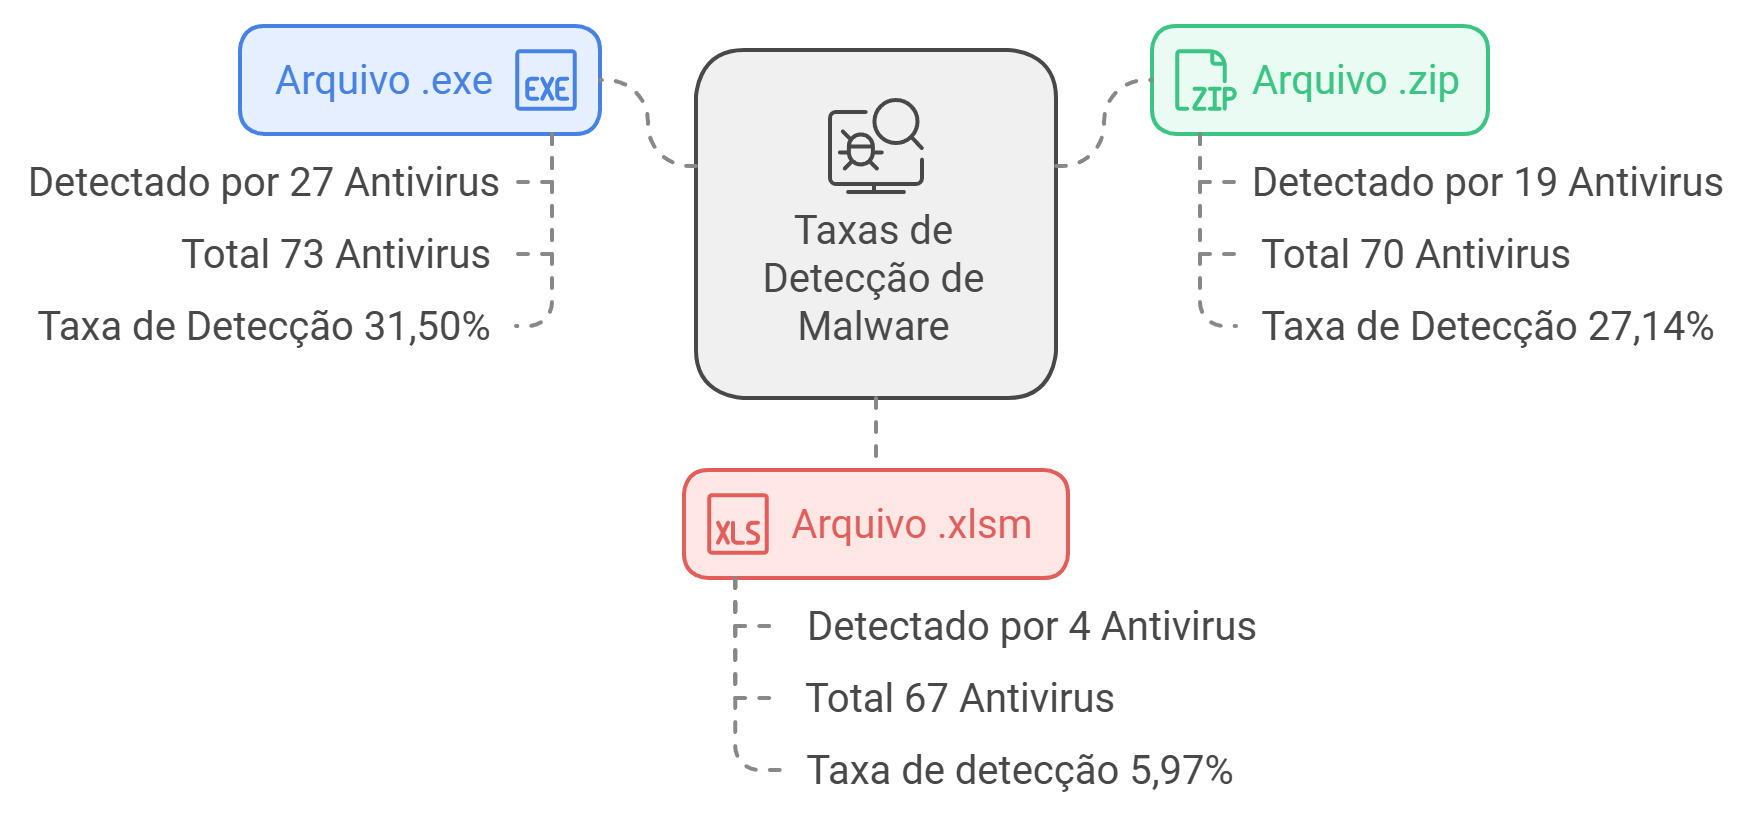
\includegraphics[width=1\textwidth]{imgs/ViruzTotal.png} % Substitua pelo caminho da imagem
\end{center}
Os resultados do VirusTotal são consistentes com testes realizados no artigo, apoiando a confiança da plataforma na detecção de \textit{malware}. A diversidade de sistemas antivírus torna o VirusTotal uma ferramenta poderosa para avaliação de ameaças.

\subsection{Tabela de resultados}
Os resultados a seguir foram obtidos a partir de testes realizados com a metodologia "Real World Prevention Test", onde cada método de infecção foi simulado cinco vezes em cada ferramenta \textit{anti-malware}, a fim de avaliar a eficiência de detecção e prevenção do \textit{keylogger}.
\begin{table}[h!]
    \centering
    \begin{tabular}{|c|c|c|c|c|}
        \hline
        \textbf{Ferramentas} & \textbf{Versão} & \textbf{.exe} & \textbf{.zip}      & \textbf{.xlsm} \\
        \hline
        Windows Defender     & 10.8750    & Sucesso       & Intermediário +    & Fracasso       \\
        \hline
        Avast                & 24.8      & Sucesso +     & Intermediário ++++ & Sucesso ++     \\
        \hline
        AVG                  & 24.8      & Sucesso +     & Intermediário ++++ & Sucesso +++    \\
        \hline
        Bit Defender         & 28.1      & Sucesso +     & Intermediário ++   & Sucesso +++    \\
        \hline
        MalwareBytes         & 5.3       & Sucesso       & Intermediário      & Sucesso ++     \\
        \hline
        Total AV             & 11.0         & Sucesso +     & Intermediário +++  & Sucesso +++    \\
        \hline
    \end{tabular}\\

    \caption{Ferramentas de detecção e suas mitigações}

    \label{tab:ferramentas}
\end{table}
\begin{flushleft}
    \textbf{Legenda:} \\
    \textbf{Sucesso} - Detectou o programa malicioso imediatamente.\\
    \textbf{Intermediário} - Detectou após múltiplas tentativas ou etapas.\\
    \textbf{Fracasso} - De forma alguma conseguiu detectar o programa malicioso.\\
    \textbf{+} - Indica maior eficiência. Quanto mais símbolos, mais rápida e eficaz é a detecção. Nenhum + indica o sistema menos eficiente, e ++++ representa o mais eficiente.
\end{flushleft}


\subsection{Observações dos resultados}
\subsubsection*{Windows Defender}
\begin{itemize}
    \item \textbf{Arquivo \texttt{.exe}}: A detecção é inconsistente. Em alguns testes, o arquivo malicioso é detectado, enquanto em outros não. No entanto, em todos os casos, a execução é bloqueada com um aviso de programa malicioso.
    \item \textbf{Arquivo \texttt{.zip}}: Não detecta o conteúdo malicioso dentro do arquivo compactado. Após a extração, a detecção é inconsistente, mas sempre bloqueia a execução com um aviso de programa malicioso.
    \item \textbf{Arquivo \texttt{.xlsm}}: Não identifica o download do arquivo malicioso feito via código VBA no \texttt{.xlsm}, permitindo sua execução sem bloqueios.
\end{itemize}

\subsubsection*{Avast}
\begin{itemize}
    \item \textbf{Arquivo \texttt{.exe}}: Detecta e bloqueia o arquivo malicioso imediatamente, impedindo o download ainda durante o processo de download do arquivo temporário. Também bloqueia posteriormente o download do arquivo \texttt{.exe} na fonte original.
    \item \textbf{Arquivo \texttt{.zip}}: Após a extração, o arquivo malicioso é detectado e colocado em quarentena, e o próprio arquivo \texttt{.zip} é colocado em quarentena após uma segunda tentativa de extração. O Avast posteriormente também bloqueia o download do \texttt{.zip} na fonte.
    \item \textbf{Arquivo \texttt{.xlsm}}:  Detecta o arquivo .exe após a execução de download do VBA e desativa futuras execuções do Macro no arquivo xlsm. Consequentimente o \textit{keylogger} não é executato.
    \item \textbf{Acesso}: Remove o acesso remoto.
\end{itemize}

\subsubsection*{AVG}
\begin{itemize}
    \item \textbf{Arquivo \texttt{.exe}}: Detecta e bloqueia o arquivo malicioso imediatamente, impedindo o download durante o processo de download do arquivo temporário. Também bloqueia o download do arquivo \texttt{.exe} na fonte original.
    \item \textbf{Arquivo \texttt{.zip}}: Após a extração, o arquivo malicioso é detectado e colocado em quarentena, e o próprio arquivo \texttt{.zip} também é colocado em quarentena após uma segunda tentativa de extração. O AVG posteriormente também bloqueia o download do \texttt{.zip} na fonte.
    \item \textbf{Arquivo \texttt{.xlsm}}: Bloqueia o acesso do código VBA aos diretórios da máquina, impedindo o download e a execução do código.
    \item \textbf{Acesso}: Remove o acesso remoto.
\end{itemize}

\subsubsection*{Bitdefender}
\begin{itemize}
    \item \textbf{Arquivo \texttt{.exe}}: Detecta e bloqueia o arquivo malicioso imediatamente, impedindo o download durante o processo de download do arquivo temporário. Também bloqueia o download do arquivo \texttt{.exe} na fonte original.
    \item \textbf{Arquivo \texttt{.zip}}: Após a extração, o arquivo malicioso é detectado e bloqueado, mas de maneira lenta, permitindo sua execução momentânea antes do bloqueio.
    \item \textbf{Arquivo \texttt{.xlsm}}: Bloqueia o acesso do código VBA aos diretórios da máquina, impedindo o download e a execução do código.
    \item \textbf{Acesso}: Remove o acesso remoto.
\end{itemize}

\subsubsection*{MalwareBytes}
\begin{itemize}
    \item \textbf{Arquivo \texttt{.exe}}: Não detecta o arquivo durante o download, mas bloqueia sua execução quando o identifica como \textit{malware}, colocando-o em quarentena.
    \item \textbf{Arquivo \texttt{.zip}}: Não detecta o conteúdo malicioso dentro do arquivo compactado durante o download ou na extração. Apenas bloqueia o arquivo \texttt{.exe} ao ser executado, colocando-o em quarentena.
    \item \textbf{Arquivo \texttt{.xlsm}}: A detecção e o bloqueio ocorrem apenas durante a execução do \texttt{.exe}. O download do \texttt{.exe} é permitido, mas sua execução é bloqueada. (Apenas na execução o arquvo é detectado) \textit{Keylogger} não é executato.
\end{itemize}

\subsubsection*{Total AV}
\begin{itemize}
    \item \textbf{Arquivo \texttt{.exe}}: Detecta e bloqueia o arquivo malicioso imediatamente, impedindo o download durante o processo de download do arquivo temporário. Também bloqueia o download do arquivo \texttt{.exe} na fonte original.
    \item \textbf{Arquivo \texttt{.zip}}: Não detecta o conteúdo malicioso durante o download. Após a extração, o arquivo malicioso é detectado e bloqueado. Não exclui o .zip e nem bloqueia seu downloand na fonte.
    \item \textbf{Arquivo \texttt{.xlsm}}: Bloqueia o acesso do código VBA aos diretórios da máquina, impedindo o download e a execução do código.
\end{itemize}

Nenhum dos programas antivírus testados detecta o arquivo \texttt{.xlsm} como malicioso, nem o conteúdo do arquivo \texttt{.zip} durante o primeiro momento de download.

\section{Conclusão}

De acordo com os resultados obtidos, verifica-se que a eficácia da proteção varia dependendo do método de infecção utilizado pelo \textit{keylogger} e do tipo de arquivos maliciosos.

\noindent\textbf{Arquivos \texttt{.exe}:} Avast, AVG e Total AV bloquearam 100\% dos arquivos, enquanto o Windows Defender teve desempenho inconsistente.

\noindent\textbf{Arquivos \texttt{.zip}:} Embora algumas ferramentas detectassem o \textit{malware} após extração, a proteção foi insuficiente durante o download do arquivo compactado.

\noindent\textbf{Arquivos \texttt{.xlsm}:} Nenhum antivírus detectou o arquivo diretamente, mas ferramentas como Avast e AVG bloquearam o código VBA malicioso subsequente.

\subsection*{Interpretação dos Dados}
A detecção eficaz depende de métodos heurísticos e comportamentais. A falha na detecção de arquivos \texttt{.zip} e \texttt{.xlsm} destaca vulnerabilidades.

\subsection*{Síntese Final}
Aplicativos como Avast, AVG e Bitdefender se destacaram na detecção de diferentes tipos de ameaças, incluindo \textit{keyloggers}, enquanto o Windows Defender demonstrou vantagens significativas, especialmente na detecção de arquivos compactados e macros. A análise do comportamento do \textit{keylogger} mostrou que:

A detecção rápida é essencial para prevenir a execução de códigos maliciosos, como keyloggers. 
O método de transferência utilizando arquivos .xlsm continua sendo uma vulnerabilidade em muitos 
programas antivírus, facilitando a propagação de keyloggers. Para o tipo de malware utilizado neste 
estudo, o resultado encontrado foi que a detecção foi mais eficaz em ferramentas com técnicas de 
heurística aprimoradas. Portanto, o estudo evidenciou a necessidade de melhorias nos métodos de detecção 
heurística, além do desenvolvimento de estratégias de conscientização do usuário para mitigar os riscos associados a keyloggers e outros arquivos maliciosos.


\bibliographystyle{plainnat}
\bibliography{sbc-template.bib}
\end{document}
